% !TeX program = xelatex
\documentclass[a4paper,10pt]{article}

% ============================================================================
% កញ្ចប់បណ្ណាល័យ (Packages) – តាមលំនាំស្តង់ដារ អនុវិទ្យាល័យព្រះក្រសាំង (ls_plan.tex)
% បរិបទ៖ ថ្នាក់រៀនគ្មានស្លាយ LCD – បង្រៀនដោយប្រើក្ដារខៀន សៀវភៅគោល និងសន្លឹកកិច្ចការស-ខ្មៅ
% ============================================================================
\usepackage[a4paper, left=0.95cm, right=0.95cm, top=0.85cm, bottom=0.92cm, footskip=0.52cm]{geometry}
\usepackage{amsmath}
\usepackage{unicode-math}
\usepackage{fontspec}
\usepackage{array, longtable, multirow, colortbl}
\usepackage[table]{xcolor}
\usepackage{enumitem}
\usepackage{pifont}
\usepackage{fancyhdr}
\usepackage{tikz}
\usetikzlibrary{calc, arrows.meta, positioning, babel}

\makeatletter
\let\@expl@@@mark@update@singlecol@structures@@\relax
\makeatother

\providecommand{\NGSFindFonts}{%
  \IfFileExists{C:/Windows/Fonts/cambria.ttc}{%
    \def\NGSSysPath{C:/Windows/Fonts/}%
    \def\NGSUserPath{C:/Users/KIT/AppData/Local/Microsoft/Windows/Fonts/}%
  }{%
    \IfFileExists{./fonts/KhmerOSsiemreap.ttf}{\def\NGSSysPath{./fonts/}\def\NGSUserPath{./fonts/}}{%
    \IfFileExists{../fonts/KhmerOSsiemreap.ttf}{\def\NGSSysPath{../fonts/}\def\NGSUserPath{../fonts/}}{%
    \IfFileExists{../../fonts/KhmerOSsiemreap.ttf}{\def\NGSSysPath{../../fonts/}\def\NGSUserPath{../../fonts/}}{%
    \IfFileExists{../../../fonts/KhmerOSsiemreap.ttf}{\def\NGSSysPath{../../../fonts/}\def\NGSUserPath{../../../fonts/}}{%
    \IfFileExists{../../../../fonts/KhmerOSsiemreap.ttf}{\def\NGSSysPath{../../../../fonts/}\def\NGSUserPath{../../../../fonts/}}{%
    \IfFileExists{../../../../../fonts/KhmerOSsiemreap.ttf}{\def\NGSSysPath{../../../../../fonts/}\def\NGSUserPath{../../../../../fonts/}}{%
    \IfFileExists{../../../../../../fonts/KhmerOSsiemreap.ttf}{\def\NGSSysPath{../../../../../../fonts/}\def\NGSUserPath{../../../../../../fonts/}}{%
      \def\NGSSysPath{../../../../../../../fonts/}\def\NGSUserPath{../../../../../../../fonts/}%
    }}}}}}}%
  }%
}
\NGSFindFonts

\setmathfont[Path={\NGSSysPath}, FontIndex=1, Scale=1.02]{cambria.ttc}
\defaultfontfeatures{Ligatures=TeX}

\setmainfont[
  Path={\NGSUserPath},
  Extension=.ttf,
  Script=Khmer,
  BoldFont={KhmerOSsiemreap},
  BoldFeatures={FakeBold=1.8},
  ItalicFont={KhmerOSsiemreap},
  ItalicFeatures={FakeSlant=0.25},
  BoldItalicFont={KhmerOSsiemreap},
  BoldItalicFeatures={FakeBold=1.8, FakeSlant=0.25}
]{KhmerOSsiemreap}

\newfontfamily\muol[Path={\NGSUserPath}, Extension=.ttf, Script=Khmer]{KhmerOSmuollight}
\newfontfamily\TimesEn[Path={\NGSSysPath}, Extension=.ttf, BoldFont={timesbd}, ItalicFont={timesi}, BoldItalicFont={timesbi}]{times}
\newfontfamily\NagaBold[Path={\NGSUserPath}, Extension=.ttf]{AKbalthom Naga Bold}
\newfontfamily\CalibriFont[Path={\NGSSysPath}, Extension=.ttf]{calibri}
\newfontfamily\Tacteing[Path={\NGSUserPath}]{TACTENG.TTF}
\newfontfamily\CourierBullet[Path={\NGSSysPath}, Extension=.ttf]{cour}
\newcommand{\wcirc}{{\CourierBullet\fontsize{9.5pt}{11pt}\selectfont o}}

\XeTeXlinebreaklocale "km"
\XeTeXlinebreakskip = 0pt plus 1pt minus 0.1pt

\definecolor{stepgray}{HTML}{D9D9D9}
\definecolor{headgray}{HTML}{F2F2F2}
\definecolor{boxgray}{HTML}{D9D9D9}
\definecolor{darkred}{HTML}{C00000}
\definecolor{red5e}{HTML}{FF0000}

\pagestyle{fancy}
\fancyhf{}
\renewcommand{\headrulewidth}{0pt}
\fancyfoot[R]{\CalibriFont\fontsize{11pt}{13pt}\selectfont\thepage}

\setlength{\parindent}{0pt}
\setlength{\parskip}{0pt}
\setlength{\tabcolsep}{3.8pt}

\newcolumntype{L}[1]{>{\raggedright\arraybackslash}p{#1}}

\newcommand{\en}[1]{{\TimesEn #1}}
\newcommand{\enbf}[1]{{\TimesEn\textbf{#1}}}
\newcommand{\unit}[1]{\,\text{\en{#1}}}
\newcommand{\fiveE}[1]{{\NagaBold\fontsize{9.5pt}{13pt}\selectfont\textcolor{red5e}{#1}}}
\newcommand{\timenote}[1]{\textcolor{darkred}{\textit{#1}}}
\newcommand{\graybox}[1]{\colorbox{boxgray}{\strut\hspace{2pt}#1\hspace{2pt}}}
\newcommand{\ditem}{\tikz[baseline=-0.5ex]\fill (0,0.42ex) -- (0.42ex,0) -- (0,-0.42ex) -- (-0.42ex,0) -- cycle;\hspace{0.3em}}
\newcommand{\cnum}[1]{{\fontsize{10.5pt}{12pt}\selectfont\ding{\numexpr171+#1\relax}}\hspace{0.2em}}
\newcommand{\cfig}[1]{\par\vspace{4pt}{\centering #1\par}\vspace{4pt}}
\newcommand{\stepheader}[1]{\multicolumn{3}{|c|}{\cellcolor{stepgray}\muol #1} \\* \noalign{\hrule height 0.4pt}}
\newcommand{\khmflourish}{{\Tacteing\fontsize{36pt}{14pt}\selectfont\raisebox{-5pt}{3}}}

% ============================================================================
% ម៉ាក្រូរូបភាពគរុកោសល្យស-ខ្មៅ (Proportional B&W TikZ Diagrams)
% ============================================================================

% ១. E1 Engage: ប្រអប់ផ្ទៃក្រឡា ២x២ សម្រាប់ផ្ទាំងរូបថតប្រាសាទ (3x+2)(x+1) (ទំ.៥៩)
\newcommand{\figEngageALGFour}{%
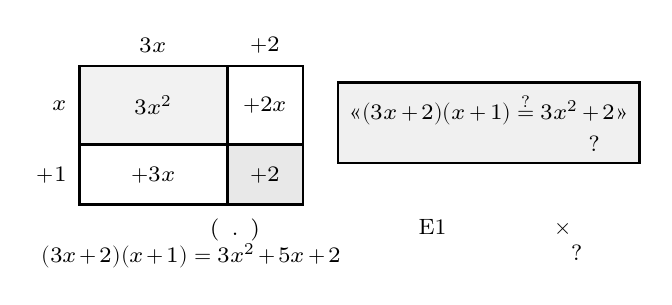
\begin{tikzpicture}[scale=0.80, every node/.style={font=\footnotesize, text=black}]
  % ឆ្វេង៖ ក្រឡាចត្រង្គផ្ទៃក្រឡា 2x2
  \begin{scope}[shift={(0,0)}]
    \draw[black, line width=1.0pt, fill=gray!10] (0,0.95) rectangle (2.35,2.20);
    \draw[black, line width=1.0pt, fill=white] (2.35,0.95) rectangle (3.55,2.20);
    \draw[black, line width=1.0pt, fill=white] (0,0) rectangle (2.35,0.95);
    \draw[black, line width=1.0pt, fill=gray!18] (2.35,0) rectangle (3.55,0.95);
    \node at (1.175,1.575) {$3x^2$};
    \node at (2.95,1.575) {$+2x$};
    \node at (1.175,0.475) {$+3x$};
    \node at (2.95,0.475) {$+2$};
    \node[above=1pt] at (1.175,2.20) {$3x$};
    \node[above=1pt] at (2.95,2.20) {$+2$};
    \node[left=1pt] at (0,1.575) {$x$};
    \node[left=1pt] at (0,0.475) {$+1$};
    \node[anchor=north, text width=3.80cm, align=center] at (1.775,-0.08) {ផ្ទៃក្រឡារូបថត (ទំ.៥៩)៖\\$(3x+2)(x+1) = 3x^2 + 5x + 2$};
  \end{scope}

  % ស្ដាំ៖ អន្ទាក់គុណតែតួមុខ និងតួក្រោយ
  \begin{scope}[shift={(4.45,0)}]
    \node[draw=black, line width=0.9pt, fill=gray!12, text width=3.55cm, align=center, inner sep=4pt] at (2.05,1.30) {
      អន្ទាក់កំហុសញឹកញាប់៖\\
      «$(3x+2)(x+1) \stackrel{?}{=} 3x^2 + 2$»\\[2pt]
      តើបាត់ផ្ទៃក្រឡាចំនួនប៉ុន្មានប្រអប់?
    };
    \node[anchor=north, text width=3.70cm, align=center] at (2.05,-0.08) {បេសកកម្ម E1៖ ហេតុអ្វីទ្វេធា $\times$ ទ្វេធា\\បង្កើតបាន ៤ តួរងមុនពេលបង្រួម?};
  \end{scope}
\end{tikzpicture}}

% ២. E4 Elaborate: ប៉ូតង់ចែកពហុធាដោយបំពេញខ្ទង់សូន្យ (x^3 + 0x^2 + 0x - 2) ÷ (x - 1) (ទំ.៦២)
\newcommand{\figPotenceALGFour}{%
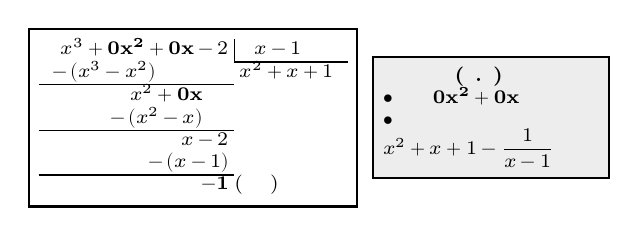
\begin{tikzpicture}[every node/.style={font=\scriptsize, text=black}]
  \node[draw=black, line width=0.9pt, fill=white, inner sep=3.5pt] (pot) at (0,0) {%
    $\begin{array}{r@{\;}l}
      x^3 + \mathbf{0x^2} + \mathbf{0x} - 2 & \multicolumn{1}{|l}{\;x - 1} \\ \cline{2-2}
      -\,(x^3 - x^2)\phantom{+0x-2} & \;x^2 + x + 1 \\ \cline{1-1}
      x^2 + \mathbf{0x}\phantom{-2} & \\
      -\,(x^2 - x)\phantom{-2} & \\ \cline{1-1}
      x - 2 & \\
      -\,(x - 1) & \\ \cline{1-1}
      \mathbf{-1} & \text{(សំណល់)}
    \end{array}$%
  };
  \node[draw=black, line width=0.75pt, fill=gray!14, text width=2.75cm, align=left, inner sep=3.5pt, right=5pt of pot] {
    \textbf{គន្លឹះប៉ូតង់ (ទំ.៦២)៖}\\
    $\bullet$ បំពេញ $\mathbf{0x^2 + 0x}$ មុនចែក\\
    $\bullet$ លទ្ធផល៖\\
    $x^2 + x + 1 - \dfrac{1}{x-1}$
  };
\end{tikzpicture}}

\begin{document}
\fontsize{10pt}{15.2pt}\selectfont

% -------------------- ក្បាលកិច្ចតែងការ (Header) --------------------
\begin{center}
  {\muol\fontsize{11pt}{16pt}\selectfont ព្រះរាជាណាចក្រកម្ពុជា}\\[2pt]
  {\muol\fontsize{10pt}{15pt}\selectfont ជាតិ សាសនា ព្រះមហាក្សត្រ}\\[1pt]
  \khmflourish
\end{center}

\vspace{-28pt}
{\muol\fontsize{9.5pt}{12.5pt}\selectfont
មន្ទីរអប់រំ យុវជន និងកីឡា ខេត្តកំពង់ធំ\\
ការិយាល័យអប់រំ យុវជន និងកីឡា ស្រុកកំពង់ស្វាយ\\
អនុវិទ្យាល័យព្រះក្រសាំង}

\vspace{1pt}
\begin{center}
  {\muol\fontsize{10pt}{14pt}\selectfont កិច្ចតែងការបង្រៀន}
\end{center}
\vspace{0pt}

% -------------------- ព័ត៌មានទូទៅ (Metadata) --------------------
{\renewcommand{\arraystretch}{0.95}
\hspace*{4.05cm}%
\begin{tabular}{@{}l l l@{}}
  - \hspace{0.35cm} មុខវិជ្ជា & : & គណិតវិទ្យា ថ្នាក់ទី៨ \\
  - \hspace{0.35cm} ចំណងជើងមេរៀន & : & មេរៀនទី៥ កន្សោមពីជគណិត \\
  - \hspace{0.35cm} ចំណងជើងរង & : & ២.៤--២.៥ វិធីគុណពហុធា និងវិធីចែកពហុធា (ទំ.៥៩--៦២) \\
  - \hspace{0.35cm} រយៈពេល & : & ១ ម៉ោងសិក្សា (៥០ នាទី) \\
  - \hspace{0.35cm} បង្រៀនដោយ & : & ហុក ប៊ុនថែន \\
  - \hspace{0.35cm} កាលបរិច្ឆេទ & : & ថ្ងៃអង្គារ ១៤រោច ខែកត្តិក ព.ស.២៥៧០ (៨ ធ្នូ ២០២៦) \\
\end{tabular}
}

\vspace{1pt}

% -------------------- I. វត្ថុបំណង --------------------
\textbf{I.} {\muol វត្ថុបំណង}\\[1pt]
\hspace*{0.55cm}%
\begin{tabular}{@{}l l L{14.2cm}@{}}
  \wcirc \hspace{0.25cm} វិជ្ជាសម្បទា & : & សិស្សប្រាប់បានត្រឹមត្រូវនូវវិធានគុណឯកធានឹងពហុធា គុណពហុធានឹងពហុធា ចែកពហុធានឹងឯកធា និងទំនាក់ទំនងចែកពហុធាមានសំណល់ $\frac{\text{តំណាងចែក}}{\text{តួចែក}} = \text{ផលចែក} + \frac{\text{សំណល់}}{\text{តួចែក}}$ តាមសៀវភៅគោល ទំ.៥៩--៦២ ។ \\
  \wcirc \hspace{0.25cm} បំណិនសម្បទា & : & សិស្សគណនាផលគុណពហុធាតាមជួរដេក/ប្រអប់ផ្ទៃក្រឡា និងតាមជួរឈរ ព្រមទាំងធ្វើប្រមាណវិធីចែកពហុធាដោយប្រើ \textbf{ប៉ូតង់បំពេញខ្ទង់សូន្យ ($0x^k$)} បានត្រឹមត្រូវ ។ \\
  \wcirc \hspace{0.25cm} ចរិយាសម្បទា & : & សិស្សមានទម្លាប់រៀបពហុធាតាមលំដាប់ដឺក្រេចុះ និងដាក់ខ្ទង់ $0x^k$ មុនធ្វើប្រមាណវិធីគុណ-ចែក ព្រមទាំងផ្ទៀងផ្ទាត់សំណល់ជាមួយដៃគូដោយហ្មត់ចត់ ។ \\
\end{tabular}

\vspace{1pt}

% -------------------- II. សម្ភារៈឧបទេស --------------------
\textbf{II.} {\muol សម្ភារៈឧបទេស}\\[1pt]
\hspace*{0.55cm}$\bullet$ \hspace{0.35cm} សៀវភៅសិក្សាគោលគណិតវិទ្យាថ្នាក់ទី៨ (ទំ.៥៩--៦២ និងទំ.៧២--៧៣) ក្ដារខៀន ដីស បន្ទាត់ និងសន្លឹកកិច្ចការសិស្សស-ខ្មៅ (\en{Worksheet\_ALG54} ចំនួន ២ ទំព័រ \en{A4} ដោយគ្មានស្លាយ \en{LCD}) ។

\vspace{1pt}

% -------------------- III. វិធីសាស្រ្តបង្រៀន --------------------
\textbf{III.} {\muol វិធីសាស្រ្តបង្រៀន}\\[1pt]
\hspace*{0.55cm}$\bullet$ \hspace{0.35cm} គោលវិធីសិស្សមជ្ឈមណ្ឌលតាមគំរូ \en{5Es} រួមបញ្ចូល \textbf{ក្រឡាប្រអប់គុណពីរវិមាត្រ និងប៉ូតង់ចែកអឺគ្លីតបំពេញខ្ទង់សូន្យ} (\en{2D Box-Grid Multiplication \& Zero-Placeholder Euclidean Potence}; \en{Marpa, 2019; Aydin-G\"u\c{c} \& Ayg\"un, 2021}) ។

\vspace{2pt}

% -------------------- IV. ដំណើរការបង្រៀន --------------------
\textbf{IV.} {\muol ដំណើរការបង្រៀន}\\[-6pt]

{\renewcommand{\arraystretch}{1.15}
\begin{longtable}{|L{5.50cm}|L{7.90cm}|L{4.80cm}|}
\hline
\multicolumn{1}{|c|}{\cellcolor{headgray}\muol សកម្មភាពគ្រូ} &
\multicolumn{1}{c|}{\cellcolor{headgray}\muol ខ្លឹមសារមេរៀន} &
\multicolumn{1}{c|}{\cellcolor{headgray}\muol សកម្មភាពសិស្ស} \\[2pt]
\hline
\endfirsthead

\hline
\multicolumn{1}{|c|}{\cellcolor{headgray}\muol សកម្មភាពគ្រូ} &
\multicolumn{1}{c|}{\cellcolor{headgray}\muol ខ្លឹមសារមេរៀន} &
\multicolumn{1}{c|}{\cellcolor{headgray}\muol សកម្មភាពសិស្ស} \\[2pt]
\hline
\endhead

\hline
\endfoot

% ==================== ជំហានទី១ (2min) ====================
\stepheader{ជំហានទី១ ៖ រដ្ឋបាលថ្នាក់ (២ នាទី)}
$\bullet$ ពិនិត្យអវត្តមាន សណ្ដាប់ធ្នាប់ អនាម័យ និងសៀវភៅគោល \par\vspace{1pt}
$\bullet$ ចែកសន្លឹកកិច្ចការស-ខ្មៅ \en{Worksheet\_ALG54} ដល់សិស្សគ្រប់គ្នា
&
$\bullet$ វត្តមានសិស្ស ឯកសណ្ឋាន និងសណ្ដាប់ធ្នាប់ថ្នាក់រៀន \par
$\bullet$ សន្លឹកកិច្ចការសិស្ស \en{Worksheet\_ALG54} (ទំព័រ ១--២) លើតុរៀងៗខ្លួន
&
$\circ$ ប្រធានថ្នាក់រាយការណ៍អវត្តមាន \par
$\circ$ សរសេរឈ្មោះលើសន្លឹកកិច្ចការ \\
\hline

% ==================== ជំហានទី២ (9min) ====================
\stepheader{ជំហានទី២ ៖ កែកិច្ចការផ្ទះ រំលឹកមេរៀនចាស់ និងភ្ជាប់បញ្ហាថ្មី (៩ នាទី)}
\ditem \textbf{កែកិច្ចការផ្ទះ ($\le 3\unit{min}$)៖} \par
$\bullet$ ហៅសិស្ស ១ រូបឡើងកែលំហាត់ ២ និង ៤ក (ទំ.៧២) លើក្ដារខៀន
&
\textbf{កំណែកិច្ចការផ្ទះ (សៀវភៅគោល ទំ.៧២)៖} \par
១) $20011 = \mathbf{2\cdot 10^4 + 0\cdot 10^3 + 0\cdot 10^2 + 1\cdot 10^1 + 1}$ ។ \par
២) $A - B = (x^4+2x^2-3x+1)-(-2x^4-3x^3+x^2-x+3) = \mathbf{3x^4 + 3x^3 + x^2 - 2x - 2}$ ។
&
$\circ$ ផ្ទៀងផ្ទាត់ការដូរសញ្ញា $-(-2x^4)=+2x^4$ និងកែចម្លើយក្នុងសៀវភៅ \\[3pt]

\ditem \textbf{រំលឹកមេរៀនចាស់ ($3\unit{min}$)៖} \par
$\bullet$ សួររំលឹកពីវិធីគុណ-ចែកឯកធា និងលក្ខណៈបំបែក $a(b+c) = ab + ac$
&
\textbf{សំណួររំលឹកមូលដ្ឋានគ្រឹះ៖} \par
១) គណនា៖ $3x^2 \cdot 4x^3 = \mathbf{12x^5}$ \quad;\quad $15x^4 \div 5x^2 = \mathbf{3x^2}$ ។ \par
២) លក្ខណៈបំបែក៖ $x(3x + 1) = x\cdot 3x + x\cdot 1 = \mathbf{3x^2 + x}$ ។
&
$\circ$ ឆ្លើយផ្ទាល់មាត់ពីការបូកនិទស្សន្តពេលគុណ និងដកនិទស្សន្តពេលចែក \\[3pt]

\fiveE{E1 - Engage} \timenote{(3 នាទី)} \par\vspace{1pt}
$\bullet$ គូសក្រឡាប្រអប់ផ្ទៃក្រឡារូបថតប្រាសាទ (ឧទាហរណ៍ទី២ ទំ.៥៩) លើក្ដារខៀន រួចឱ្យសិស្សគូសធីកទស្សន៍ទាយក្នុងផ្នែកទី១
&
\textbf{ស្ថានភាពភ្ជាប់បញ្ហា៖ ផ្ទៃក្រឡារូបថតប្រាសាទ និងអន្ទាក់គុណទ្វេធា!} \par
រូបថតប្រាសាទមួយផ្ទាំងមានរាងចតុកោណកែងបណ្ដោយ $(3x+2)\unit{m}$ និងទទឹង $(x+1)\unit{m}$ (ទំ.៥៩) ។ សិស្សម្នាក់គុណតែ «តួមុខនឹងតួមុខ» និង «តួក្រោយនឹងតួក្រោយ» បាន $(3x+2)(x+1) = 3x^2 + 2$! \par
\hspace*{0.3em}– \textbf{សំណួរបេសកកម្ម៖} «តើផ្ទៃក្រឡាពិតស្មើ $3x^2+2$, ស្មើ $3x^2+3x+2$ ឬស្មើ $\mathbf{3x^2+5x+2}$? តើគាត់ភ្លេចប្រអប់រងណាខ្លះ?»
&
$\circ$ សង្កេតក្រឡាប្រអប់ $2\times 2$ លើក្ដារខៀន \par
$\circ$ គូសធីកការទស្សន៍ទាយមុនរៀនក្នុងផ្នែកទី១ នៃសន្លឹកកិច្ចការ \\[3pt]

& \cfig{\figEngageALGFour} & \\
\hline

% ==================== ជំហានទី៣ (17min) ====================
\stepheader{ជំហានទី៣ ៖ មេរៀនថ្មី — វិធីគុណពហុធា និងវិធីចែកពហុធា (១៧ នាទី)}
\fiveE{E2 - Explore} \timenote{(11 នាទី)} \par\vspace{1pt}
\ditem \textbf{សកម្មភាពទី១៖ រុករកវិធីគុណពហុធាតាមប្រអប់ផ្ទៃក្រឡា ($5.5\unit{min}$)៖} \par
$\bullet$ ឱ្យសិស្សធ្វើការជាដៃគូលើ \textbf{ផ្នែកទី២ (ក)} នៃ \en{Worksheet\_ALG54} ដើម្បីគណនា $x(3x+1)$ និង $(3x+2)(x+1)$ តាមប្រអប់ផ្ទៃក្រឡា (ទំ.៥៩)
&
\textbf{ការរុករកទី១ (២.៤ វិធីគុណពហុធា ទំ.៥៩--៦០)៖} \par
$\bullet$ \textbf{ឯកធា $\times$ ពហុធា៖} $x(3x+1) = x(3x) + x(1) = \mathbf{3x^2 + x}$ ។ \par
$\bullet$ \textbf{ពហុធា $\times$ ពហុធា៖} ក្នុងប្រអប់ $2\times 2$ គេបាន ៤ តួរងគឺ $3x(x) + 3x(1) + 2(x) + 2(1) = 3x^2 + 3x + 2x + 2 = \mathbf{3x^2 + 5x + 2}$ (បើគុណតែ $3x^2+2$ គឺបាត់តួឆ្វែង $+3x$ និង $+2x$!) ។
&
$\circ$ បំពេញប្រអប់ផ្ទៃក្រឡាទាំង ៤ ក្នុងសន្លឹកកិច្ចការ \par
$\circ$ រកឃើញតួកណ្ដាល $+3x + 2x = +5x$ ដែលសិស្សក្នុង E1 បានភ្លេច \\[3pt]

\ditem \textbf{សកម្មភាពទី២៖ រុករកវិធីចែកពហុធាដាច់ និងចែកមានសំណល់ ($5.5\unit{min}$)៖} \par
$\bullet$ ឱ្យដៃគូបន្តបំពេញ \textbf{ផ្នែកទី២ (ខ)}៖ ចែក $(15x^4-30x^6)\div 5x^2$ (ទំ.៦០) និងប៉ូតង់ចែក $(x^2-7x+10)\div(x-2)$ ធៀបនឹង $(x^2-2x+4)\div(x-1)$ (ទំ.៦១)
&
\textbf{ការរុករកទី២ (២.៥ វិធីចែកពហុធា ទំ.៦០--៦១)៖} \par
$\bullet$ \textbf{ពហុធា $\div$ ឯកធា៖} $\dfrac{15x^4 - 30x^6}{5x^2} = \dfrac{15x^4}{5x^2} - \dfrac{30x^6}{5x^2} = \mathbf{3x^2 - 6x^4}$ ។ \par
$\bullet$ \textbf{ពហុធា $\div$ ពហុធា៖} $(x^2-7x+10)\div(x-2) = \mathbf{x - 5}$ (សំណល់ $0 \implies$ \textbf{ចែកដាច់}); ចំណែក $(x^2-2x+4)\div(x-1)$ បានផលចែក $x-1$ និងសំណល់ $\mathbf{3} \implies \dfrac{x^2-2x+4}{x-1} = \mathbf{x - 1 + \dfrac{3}{x-1}}$ ។
&
$\circ$ ចែកគ្រប់តួនៃពហុធានឹងឯកធា $5x^2$ \par
$\circ$ អនុវត្តជំហាន «ចែក–គុណ–ដក–ទម្លាក់ចុះ» ក្នុងប៉ូតង់ទាំងពីរ \\[3pt]

\fiveE{E3 - Explain} \timenote{(6 នាទី)} \par\vspace{1pt}
$\bullet$ ហៅតំណាងដៃគូឡើងបកស្រាយវិធានគុណពហុធា រួចគ្រូសង្ខេបធនាគារហេតុផល \cnum{1}--\cnum{2} លើក្ដារខៀន
&
\textbf{សង្ខេបខ្លឹមសារគោល៖ ២.៤--២.៥ គុណ និងចែកពហុធា (ទំ.៥៩--៦១)} \par
$\bullet$ \textbf{វិធីគុណ (\cnum{1}--\cnum{2})៖} គុណឯកធានឹងតួនីមួយៗនៃពហុធា រួចបង្រួម (\cnum{1}); គុណកត្តានីមួយៗនៃពហុធាទី១ ទៅគ្រប់តួនៃពហុធាទី២ រួចបង្រួមឯកធាដូចគ្នា (\cnum{2}) ។
&
$\circ$ ឡើងបកស្រាយវិធានគុណពហុធាលើក្ដារខៀន \\[3pt]

$\bullet$ សង្ខេបវិធានចែកពហុធាដាច់ និងចែកមានសំណល់ (\cnum{3}--\cnum{5}) លើក្ដារខៀន
&
$\bullet$ \textbf{វិធីចែក (\cnum{3}--\cnum{5})៖} ចែកពហុធានឹងឯកធា គឺចែកគ្រប់តួនឹងឯកធានោះ (\cnum{3}) ។ មុនចែកប៉ូតង់ ត្រូវរៀបដឺក្រេចុះ និង \textbf{ដាក់ខ្ទង់ $0x^k$} ត្រង់ដឺក្រេដែលបាត់ (\cnum{4}) ហើយសរសេរ $\dfrac{\text{តំណាងចែក}}{\text{តួចែក}} = \text{ផលចែក} + \dfrac{\text{សំណល់}}{\text{តួចែក}}$ (\cnum{5}) ។
&
$\circ$ កត់ត្រាវិធាន \cnum{1}--\cnum{5} ចូលក្នុងប្រអប់ផ្នែកទី៣ នៃសន្លឹកកិច្ចការ \\
\hline

% ==================== ជំហានទី៤ (20min) ====================
\stepheader{ជំហានទី៤ ៖ ពង្រីកចំណេះដឹង និងវាយតម្លៃលទ្ធផលសិក្សា (២០ នាទី)}
\fiveE{E4 - Elaborate} \timenote{(10 នាទី)} \par\vspace{1pt}
\ditem \textbf{លំហាត់គំរូគុណពហុធាតាមជួរដេក និងជួរឈរ (ទំ.៦០, $4.5\unit{min}$)៖} \par
$\bullet$ ដឹកនាំសិស្សដោះស្រាយលំហាត់គំរូ ១ និង ២ (ទំ.៦០) ក្នុង \textbf{ផ្នែកទី៤ (១)} នៃសន្លឹកកិច្ចការ ដោយសង្កត់ធ្ងន់លើការរៀបលំដាប់ $1+x^2-3x \to x^2-3x+1$ មុនគុណជួរឈរ
&
\textbf{លំហាត់គំរូគុណពហុធា (សៀវភៅគោល ទំ.៦០)៖} \par
$\bullet$ គំរូទី១៖ $3x^2(4x^3 + xy - 5y^2) = \mathbf{12x^5 + 3x^3y - 15x^2y^2}$ ។ \par
$\bullet$ គំរូទី២ (ជួរឈរ)៖ រៀប $(x^2 - 3x + 1) \times (2x - 3)$ ៖ \par
\hspace*{0.3em}– ជួរទី១៖ $(2x)(x^2 - 3x + 1) = 2x^3 - 6x^2 + 2x$ \par
\hspace*{0.3em}– ជួរទី២៖ $(-3)(x^2 - 3x + 1) = -3x^2 + 9x - 3$ \par
\hspace*{0.3em}– បូកតម្រឹមដឺក្រេ៖ បានផលគុណ $\mathbf{2x^3 - 9x^2 + 11x - 3}$ ។
&
$\circ$ រៀបដឺក្រេចុះ $x^2-3x+1$ រួចគុណតាមជួរឈរលើសន្លឹកកិច្ចការ \\[3pt]

\ditem \textbf{លំហាត់គំរូចែកពហុធាបាត់ខ្ទង់ (ទំ.៦២) និងឆ្លុះបញ្ចាំង ($5.5\unit{min}$)៖} \par
$\bullet$ ដឹកនាំសិស្សធ្វើប៉ូតង់ចែកលំហាត់គំរូ ១ និង ២ (ទំ.៦២) ដែលបាត់ខ្ទង់ដឺក្រេកណ្ដាល និងផ្ទៀងផ្ទាត់សំណល់
&
\textbf{លំហាត់គំរូចែកពហុធាមានខ្ទង់បាត់ (សៀវភៅគោល ទំ.៦២)៖} \par
$\bullet$ គំរូទី១៖ $(8y^3 + 4y^2 + \mathbf{0y} - 7)\div(2y + 3) = \mathbf{4y^2 - 4y + 6 - \dfrac{25}{2y+3}}$ ។ \par
$\bullet$ គំរូទី២៖ $(x^3 + \mathbf{0x^2} + \mathbf{0x} - 2)\div(x - 1) = \mathbf{x^2 + x + 1 - \dfrac{1}{x-1}}$ ។ \par
$\bullet$ \textbf{ឆ្លុះបញ្ចាំង៖} ផ្ទៀងផ្ទាត់ $(x-1)(x^2+x+1) + (-1) = (x^3 - 1) - 1 = x^3 - 2$ ពិត!
&
$\circ$ សរសេរ $+0y$ និង $+0x^2+0x$ ចូលក្នុងប៉ូតង់មុនចែក \par
$\circ$ ផ្ទៀងផ្ទាត់ «តួចែក $\times$ ផលចែក $+$ សំណល់ $=$ តំណាងចែក» \\[3pt]

& \cfig{\figPotenceALGFour} & \\[3pt]

\fiveE{E5 - Evaluate} \timenote{(10 នាទី)} \par\vspace{1pt}
\ditem \textbf{អនុវត្ត «ប្រតិបត្តិ» គុណ និងចែកពហុធា (ទំ.៦០, ៦២ — $6.5\unit{min}$)៖} \par
$\bullet$ ឱ្យសិស្សធ្វើលំហាត់ \textbf{ប្រតិបត្តិគុណ} (ទំ.៦០) ដោយខ្លួនឯងក្នុងផ្នែកទី៥ (១) នៃសន្លឹកកិច្ចការ
&
\textbf{ចម្លើយលំហាត់ «ប្រតិបត្តិ» (សៀវភៅគោល ទំ.៦០ និងទំ.៦២)៖} \par
១) \textbf{ផលគុណពហុធា (ទំ.៦០)៖} ក) $2x^2(2x^2+3x-1) = \mathbf{4x^4 + 6x^3 - 2x^2}$ \;;\; ខ) $ab^2(a^2+2ab+a) = \mathbf{a^3b^2 + 2a^2b^3 + a^2b^2}$ \;;\; គ) $(a^2+2ab)(a-b) = \mathbf{a^3 + a^2b - 2ab^2}$ \;;\; ង) $\frac{1}{2}xy^2(\frac{2}{3}xy-3) = \mathbf{\frac{1}{3}x^2y^3 - \frac{3}{2}xy^2}$ ។
&
$\circ$ គណនាផលគុណពហុធា និងបង្រួមតួដូចគ្នា $2a^2b - a^2b = +a^2b$ \\[3pt]

$\bullet$ ឱ្យសិស្សបន្តធ្វើ \textbf{ប្រតិបត្តិចែក} ទាំង ៤ លំហាត់ (ទំ.៦២) រួចប្ដូរសន្លឹកកិច្ចការផ្ទៀងជាដៃគូ
&
២) \textbf{ផលចែកពហុធា (ទំ.៦២)៖} \par
\hspace*{0.3em}– ក) $(a^2b^3 + 2ab)\div(ab) = \mathbf{ab^2 + 2}$ \par
\hspace*{0.3em}– ខ) $(5x^2y^4 + 2x^3y^5 - 12x^2y^2)\div(x^2y^2) = \mathbf{5y^2 + 2xy^3 - 12}$ \par
\hspace*{0.3em}– គ) $(6x^2 + 5x - 4)\div(2x - 1) = \mathbf{3x + 4}$ (សំណល់ $0$) \par
\hspace*{0.3em}– ឃ) $(a^2 + 6a - 55)\div(a - 5) = \mathbf{a + 11}$ (សំណល់ $0$) ។
&
$\circ$ ប្ដូរសន្លឹកកិច្ចការផ្ទៀងផ្ទាត់តួ $+2$ ក្នុង $(2ab)\div(ab)=2$ និងប៉ូតង់ គ--ឃ (\en{Pause-Review}) \\[3pt]

\ditem \textbf{បិទបេសកកម្ម E1 និងតេស្តរហ័ស \en{Exit Check} ($3.5\unit{min}$)៖} \par
$\bullet$ សួរបិទបេសកកម្មផ្ទៃក្រឡារូបថត និងឱ្យសិស្សគូសរង្វង់ជម្រើស \en{A--D}
&
$\bullet$ \textbf{បិទបេសកកម្ម E1៖} ផ្ទៃក្រឡារូបថតគឺ $(3x+2)(x+1) = \mathbf{3x^2 + 5x + 2}$ ។ \par
$\bullet$ \textbf{Exit Check៖} តើផលគុណ $(2x - 3)(x + 4)$ ស្មើនឹងពហុធាមួយណា? \par
\en{A.} $2x^2 - 12$ \quad \en{B.} $2x^2 + 11x - 12$ \quad \graybox{\enbf{C.} $2x^2 + 5x - 12$ \ding{51}} \quad \en{D.} $2x^2 - 5x - 12$
&
$\circ$ គណនា $8x - 3x = +5x$ រួចគូសរង្វង់ជម្រើស \textbf{C} \\
\hline

% ==================== ជំហានទី៥ (<=2min) ====================
\stepheader{ជំហានទី៥ ៖ កិច្ចការផ្ទះ និងបណ្ដាំផ្ញើ ($\le$ ២ នាទី)}
$\bullet$ កត់ត្រាកិច្ចការផ្ទះលើក្ដារខៀន (មានបោះពុម្ពស្រាប់នៅផ្នែកទី៦ នៃសន្លឹកកិច្ចការទំព័រទី២) \par
$\bullet$ រំលឹកឱ្យប្រយ័ត្នសញ្ញាដកមុខកត្តា $-b(a-x)$ ក្នុងលំហាត់ទី៦
&
\textbf{កិច្ចការផ្ទះ (សៀវភៅសិក្សាគោល ទំ.៧២--៧៣)៖} \par
១. \textbf{លំហាត់ទី៣ គ (ទាំង ២ ឃ្លា ទំ.៧២)៖} គណនា $(x^2 + 2y)(x + 1)$ និង $(x^2 - y)(y - 4)$ ។ \par
២. \textbf{លំហាត់ទី៦ (ទំ.៧៣)៖} គណនា បង្រួម និងរៀបតាមលំដាប់ដឺក្រេចុះ៖ $a(x - b) - b(a - x) + x(a + b)$ ។ \par
៣. \textbf{លំហាត់ទី៧ ក--ខ (ទំ.៧៣)៖} គណនា និងបង្រួម៖ ក) $y(x+a-y) - a(x+y-a) - a(a^2+y^2)$ \;;\; ខ) $(t-1)(t-2) - (t+1)(t-3) - 2(t-2)(t+3)$ ។
&
$\circ$ កត់ត្រាកិច្ចការផ្ទះ និងទុកដាក់សន្លឹកកិច្ចការក្នុងសឺមីគណិតវិទ្យា \\[3pt]

$\bullet$ ណែនាំឱ្យអានចំណុច ៣.១ ជាមុនសម្រាប់ម៉ោងក្រោយ
&
$\bullet$ \textbf{អានជាមុន៖} ចំណុច \textbf{៣.១ សមភាពសំខាន់ៗ — ពន្លាតការេនៃទ្វេធា និងផលគុណទ្វេធាឆ្លាស់សញ្ញា} (សៀវភៅគោល ទំព័រ ៦៣--៦៦) ។
&
$\circ$ ទទួលបណ្ដាំផ្ញើ និងជម្រាបលាគ្រូ \\

\end{longtable}
}

\vspace{6pt}

% -------------------- ហត្ថលេខា (Signature Block) --------------------
\begin{flushright}
\begin{minipage}{9.6cm}
\centering
ថ្ងៃអង្គារ ១៤រោច ខែកត្តិក ឆ្នាំមមី អដ្ឋស័ក ពុទ្ធសករាជ ២៥៧០\\[2pt]
ព្រះក្រសាំង, ថ្ងៃទី៨ ខែធ្នូ ឆ្នាំ២០២៦\\[4pt]
{\muol គ្រូបង្រៀន}\\[32pt]
\hfill{\muol ហុក ប៊ុនថែន}\hspace*{1.4cm}
\end{minipage}
\end{flushright}

\end{document}
